\subsection{Syntax units}
\begin{figure}[b]
\centering
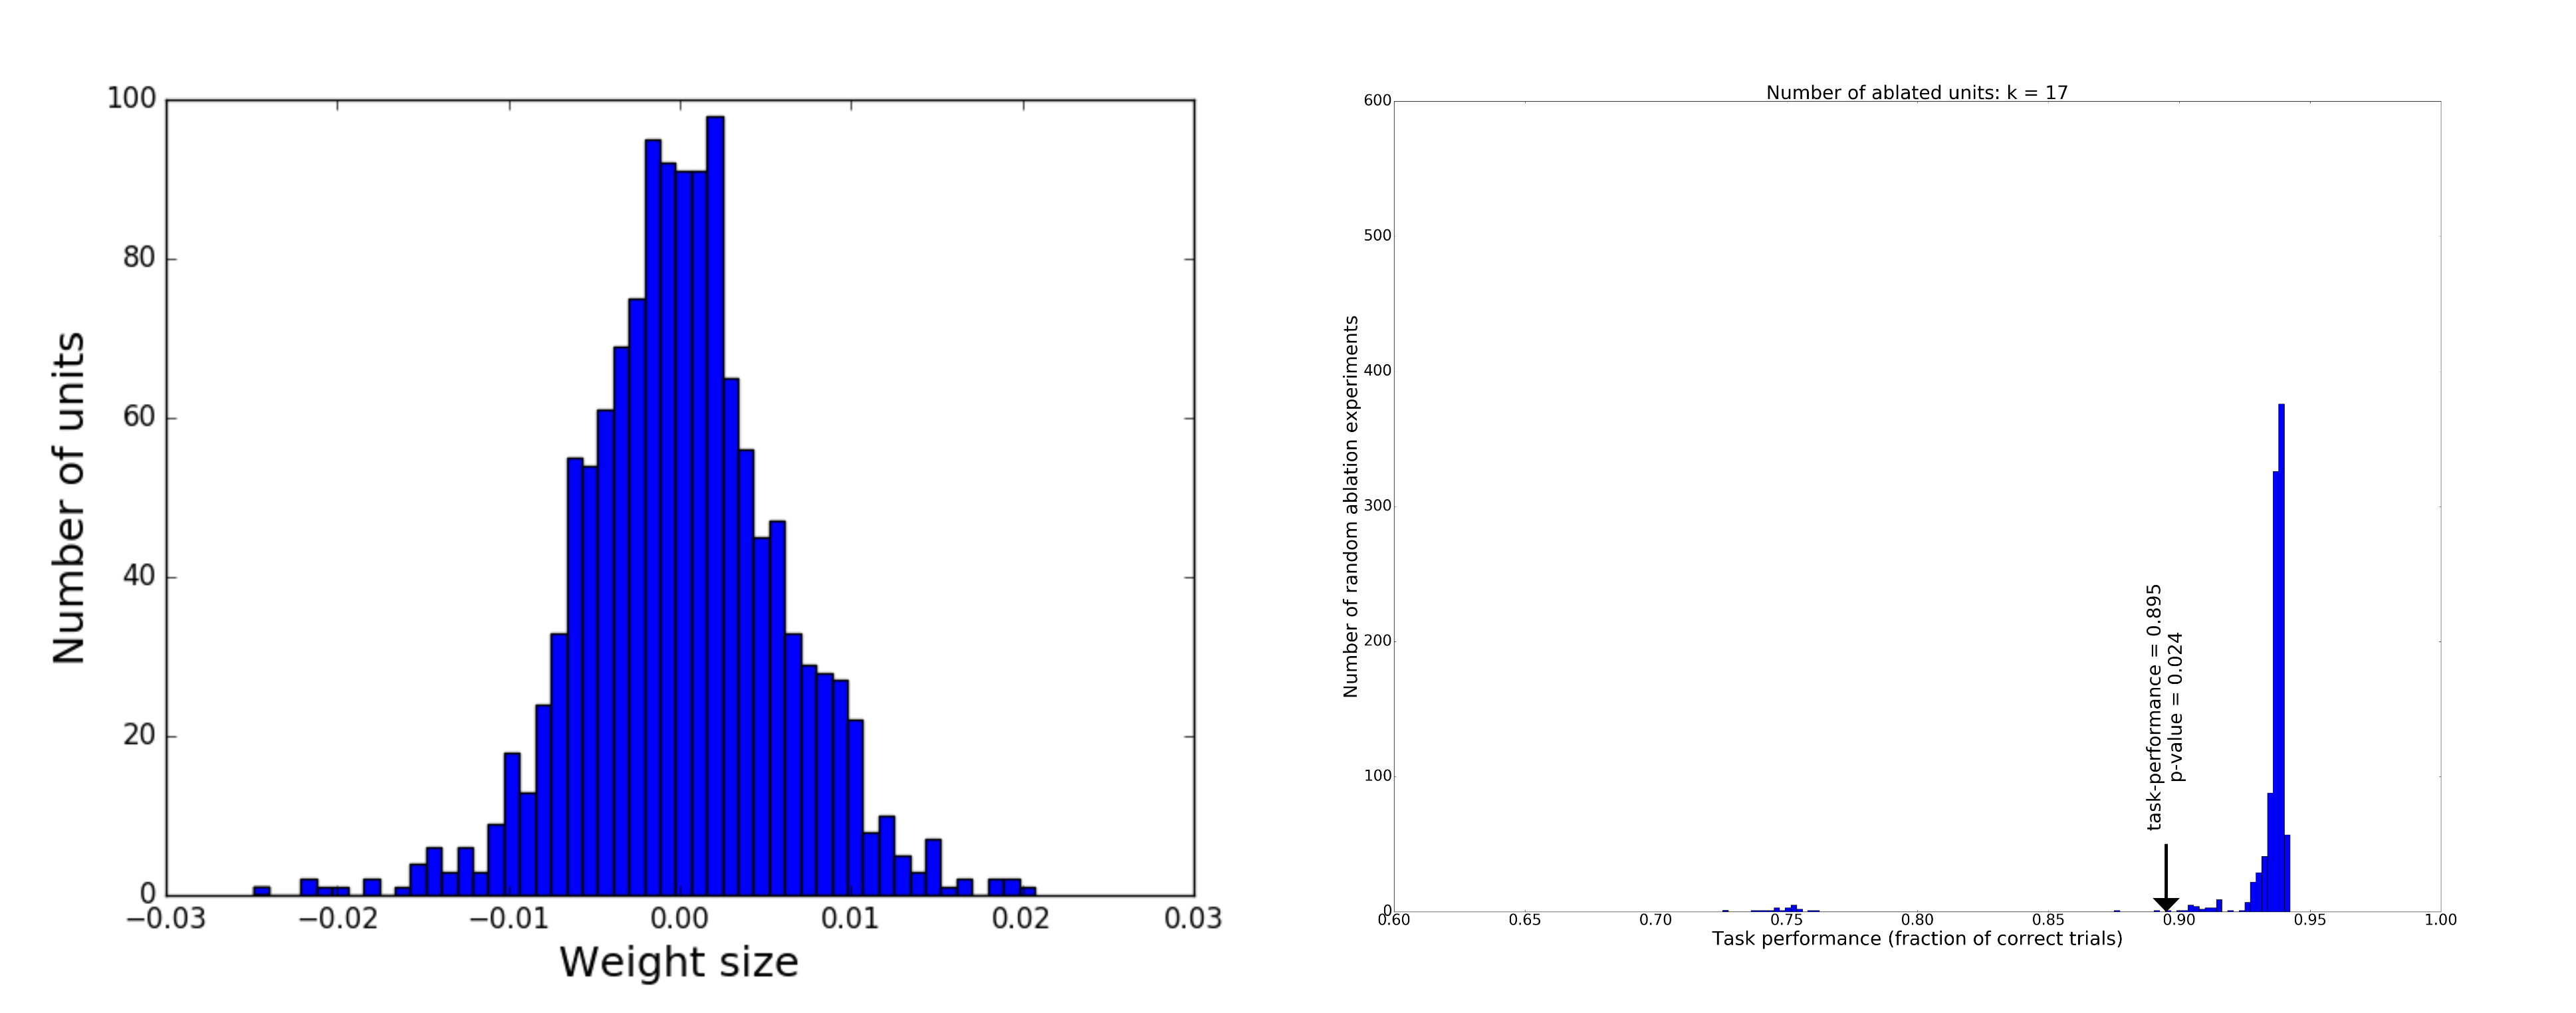
\includegraphics[width=\linewidth]{Figures/Figure6_regression.png}
\caption{(A) Distribution of the resulting weight values from the tree-depth regression model. Outlier weights were defined as having a value that is distant from the mean by more than three standard deviations (17 outlier weights in total - marked in red). (B) Task performance of 1000 models after ablating 17 random units (in blue) and based on the 17 outlier weights from the tree-depth regression model (black arrow). The reduction in performance due to outlier-weights ablation is statistically significant ($p-value < 0.05$) when compared to the null distribution generated by the random ablations.}
\end{figure}

In the previous section, a small number of units in the network was identified, which was found to store grammtical number for long-range dependecies also in the presence of interfering nouns. Remarkably, information about the two possible values of grammatical number, singluar and plural, is steadily carried by two specialized units in the network: unit 776 and 998. It remains unclear, however, how is the timing of storing and updating of number information in these units controlled by the network. In particular, given that the storage of information is controlled by the input and forget gates, how is the timing of these gates controlled by the network. To approach this, we hypothesized that other units in the network may encode information about the syntactic structure of the sentence, which could be then propagated to LR number units at the crucial moments required to successfully accomplish the NA-task. 

<<<<<<< HEAD
To uncover such units, we tested whether there are units in the network from which syntactic information can be decoded. Given that ablation of single units in the network revealed number units only, we concluded that syntactic information may be encoded by the network in a more distributed way. We therefore tested decoding from the joint activity of a group of units in the network, using a regression model trained to predict syntactic information from activity patterns of the entire network. Specifically, the dependent variable of the model was syntactic complexity, quantified by counting the number of open nodes in the syntactic-tree, referred to also as \textit{syntactic-tree depth} (section 3.2), inspired by \textcolor{red}{cite Nelso et. al 2017}. We then used the activity of all units in the network as predictors in the model, together with word frequency as a covariate. In addition, to address possible co-linearities among unit activities, and to examine from which units syntactic-tree depth can be best predicted, we used L1-regularization (section 4.2 for details). 
=======
To identify such units, we tested whether there are units in the network from which syntactic information can be decoded. Given that ablation of single units in the network revealed number units only, we concluded that syntactic information may be encoded by the network in a more distributed way. We therefore tested decoding from the joint activity of a group of units in the network, using a regression model to predict syntactic information from the pattern of activity in the entire network. Specifically, the dependent variable of the model was syntactic complexity, which was quantified by counting the number of open nodes in the syntactic-tree, inspired by \textcolor{red}{cite Nelso et. al 2017}. In what follows, we refer to the number of open nodes in the syntactic tree as \textit{syntactic-tree depth}. We then used the activity of all units in the network as predictors in the model, together with word frequency as a covariate. In additoin, to address possible co-linearities among unit activities, and to examine from which units syntactic-tree depth can be best predicted, we L1-regularized the regression model (section 4.2 for details \textcolor{red}{section 4.2 should explain that the model was trained on the data from 3.2, word frequency, standarization of the values, etc.}). 
>>>>>>> f4f6485f41ba8a2d0aa03aa24c6ed0853de36aa6

Figure 5A shows the resulting weights of all predictors in the model. We define an \textit{outlier weight} a weight whose value is more than three standard-deviations away from the mean weight size \textcolor{red}{add mean and std values}. 17 outlier weights were found in the model \textcolor{red}{?add resulting unit numbers?}, whose corresponding units may thus be carrying syntactic information, given their high weight in predicting syntactic complexity. To test this, we ran an ablation study, assuming that if these units carry syntactic information then ablating them would lead to a reduction in network performance on the NA-task compared to random ablations \textcolor{red}{We used Linzen for this. Do we want to also test of nounPP, etc?}. Figure 5B presentes the null-distribution of network performance on the NA-task, generated from 1000 ablation experiments, where in each experiment 17 random units are ablated. The black arrow represents points to the reduction in network performance when the 17 units from the regression model are ablated, which was found to be significant ($p-value=0.024$). Taken together, these results suggest that the 17 units identified by the regression model carry syntactic information required for succesfully performaing the NA-task. In what follows, we refer to these units as \textit{syntax units}.

Next, we looked into the dynamics of these units by visualizing their gate and cell dynamics during the processing of sentences with various syntactic structures. In particular, we found that unit 1150, which resulted with the highest weight in the regression study seems to have an interpretable dynamics during the processing of various types of sentences. Figure 2 \& 3 show the hidden and cell activity of this unit in the nounPP, subjrel, objrel and double-subjrel tasks. In all these cases, the activity of this unit follows the structure of the embedded phrase within the main subject-verb dependency. The hidden-variable activity of this unit is positive during the processing of the embbeded phrase and transitions to a negative value at the time when the main verb is presented, but not before it, even if other verbs preceded it (as in the case of relative clauses - Figre X\&Y). This suggests that unit 1150 can be interpreted as encoding the existence of an embedded phrase withing the long-range subject-verb dependency of the sentence. Interestingly, the cell activity of this unit consistenly increased during the procesding of the embedded phrase, similarly to what was observed in several electrodes in the language network in intracranial studies on sentence processing \textcolor{red}{cite nelson 2017 - refer to figure. TODO: for this, also add to our figures the cell activity of unit 1150}. In the next section, we show how these dynamics of unit 1150 are important for controlling the timing of gate activity in the LR number units.



\textcolor{red}{?Do we also want to note that unit 1150 had a (small) effect also on the NA-task when ablated alone...?}



